\documentclass{article}
\usepackage[utf8]{inputenc}
\usepackage{graphicx}

\title{My first open source contribution.}
\author{Marietta Lazana - t8160057@aueb.gr}
\date{May 2019}

\begin{document}

\maketitle

% Here is the abstract.
\begin{abstract}
Contributing to an open source project has proven to be extremely beneficial. It, greatly, reduced inhibitory factors by demystifying the contributory process. Personally, it was a challenge, to examine my abilities and strengths in a quite big and very fast moving project. Facing the real world of Software Engineering was surely a great experience!
  
\end{abstract}
%---

\section*{Introduction}
The "Software Engineering in Practise" course is one of the most important in my undergraduate degree, since it has prompted me to gain my first serious experience in this field. Under the supervision of the professor Diomidis Spinellis and the help of PhD candidate Antonis Gkortzis I gained useful knowledge in software engineering that broaden my horizons in this field. I learned about software design, construction, testing, maintenance, management and more, following the book of IEEE "SWEBOK, Software Engineering  Body of Knowledge". Last but not least, I gained valuable experience with version control systems by using git on a daily bases.

\section{Project Understanding}

% Image
\begin{figure}[tph!]
\centerline{
\includegraphics[totalheight=2cm]{logo.png}}
    \caption{ArchiveBox logo}
    \label{fig:verticalcell}
\end{figure}
%-----

I had two criteria while searching for a project. The first was high difficulty and the second was to be something that will excite me. So when I found ArchiveBox I thought that it was a great idea considering the level of difficulty. So I was sure that this was going to be a challenging project that will definitely help me improve.

ArchiveBox[1] is a very promising and upcoming project created by Nick Sweeting (GitHub: pirate) and has a vision of archiving everything from the internet. It is motivated by the fact that many people find interesting information on the internet that want to store locally, and most importantly, in multiple redundant common formats(HTML, PDF, PNG, WARC etc.). So, the user gives specific terminal commands including the URL that wants to archive, and then all the formats of the archived website are stored and organized in an HTML page.

While trying to build the project I faced a very basic problem. My operating system (Windows) couldn't support the project. So I came up with the solution of working from a virtual machine that runs on Linux, more precisely I worked with Oracle's VM, virtualbox. 

Finally, in order to understand deeper the project I started reading the code of every file and categorize it depending on it's role. Of course, the documentation helped me a lot in this process.


\section{My contribution}

At first, I was trying to find something that I could contribute. Luckily, the person who ones repository, Nick, mentioned me in a issue with medium difficulty.
% Image
\begin{figure}[tph!]
\centerline{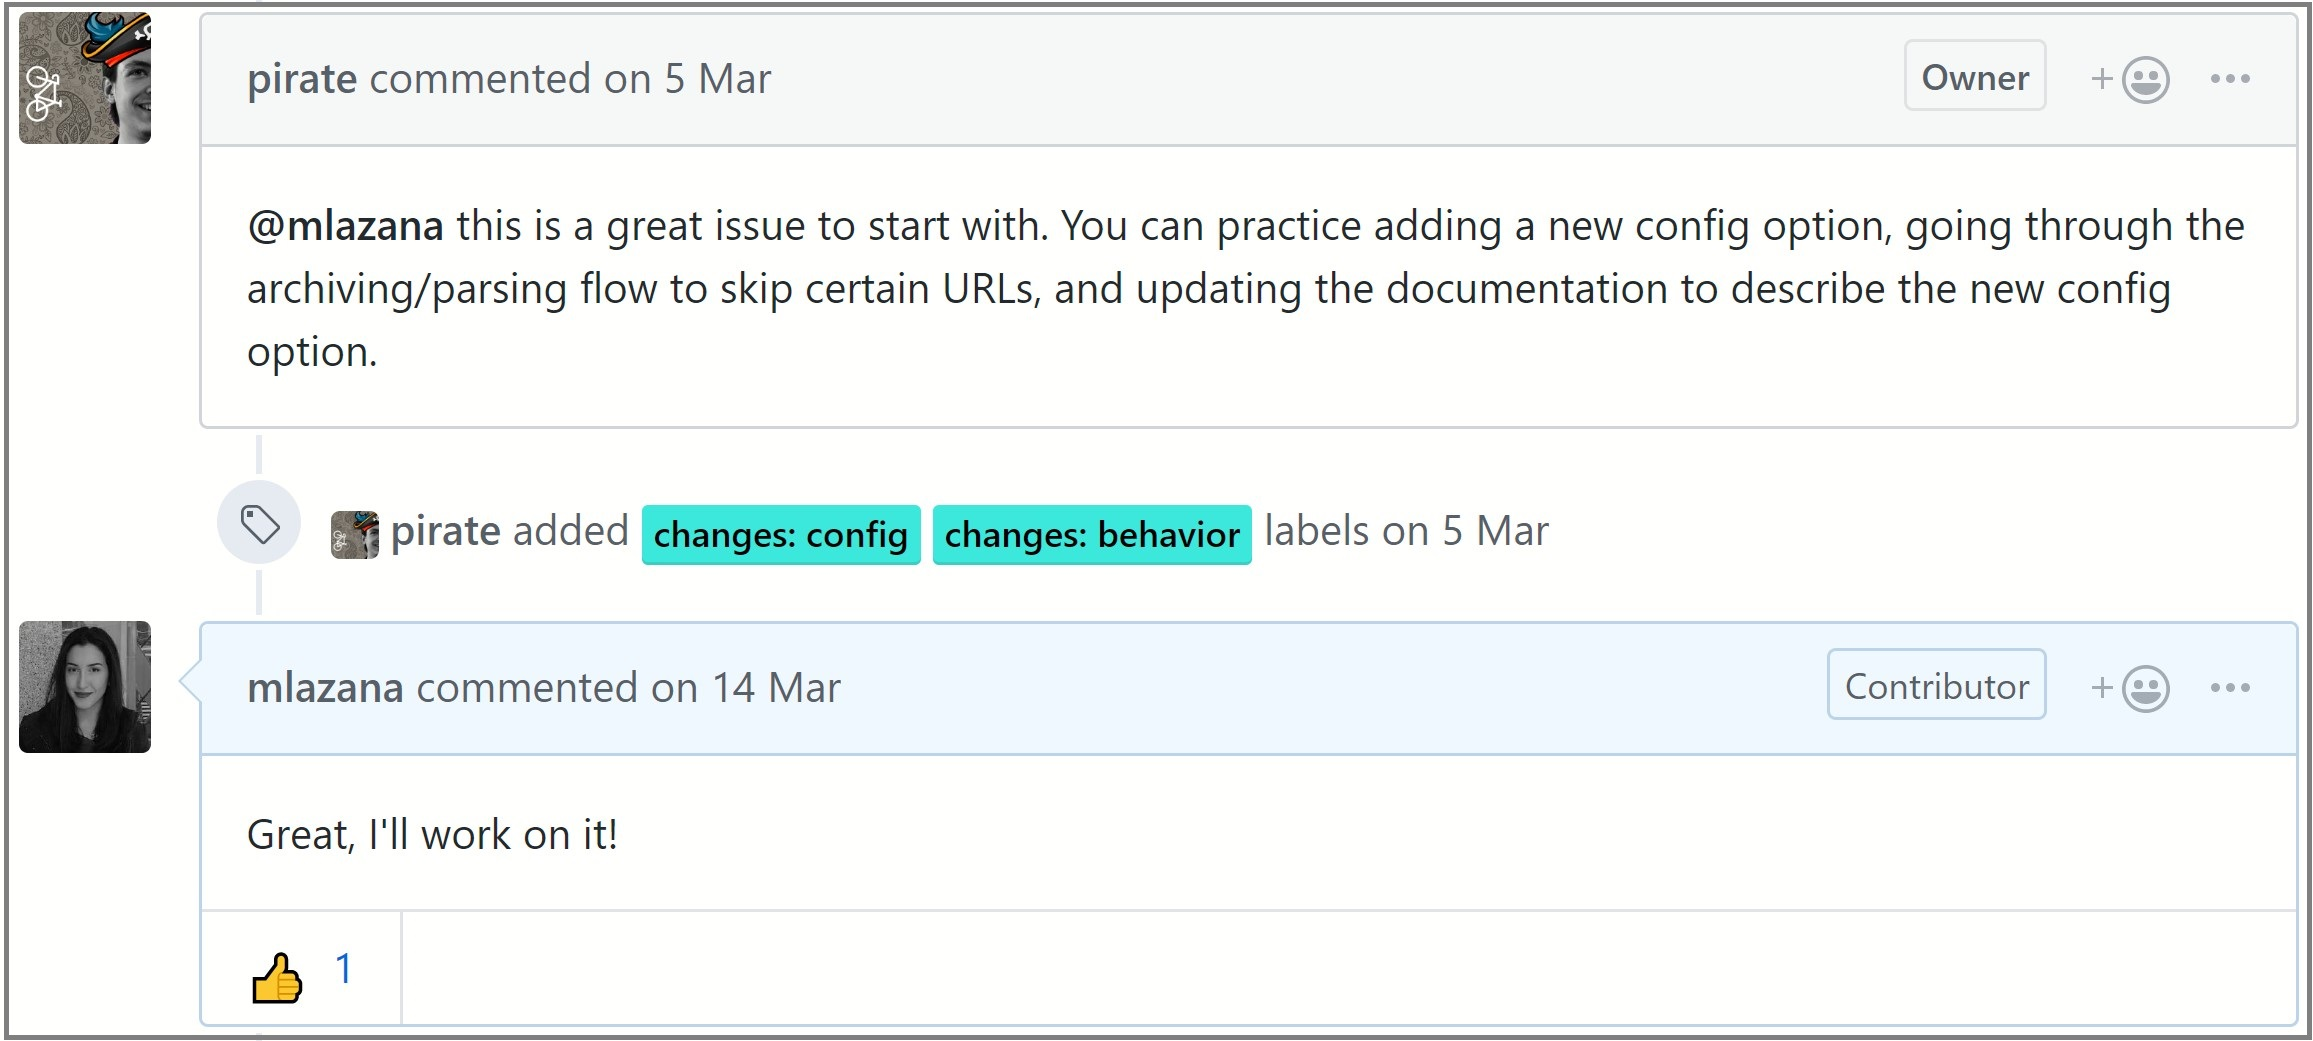
\includegraphics[totalheight=4.5cm]{mention.jpg}}
    \caption{Mentioned in issue \#200}
    \label{fig:verticalcell}
\end{figure}
%-----
That was very good for me because I needed to break out of my comfort zone and deal with a problem I didn't choose.

The issue was about creating a blacklist of URLs that shouldn't be archived. For example, when someone wanted to archive automatically his/hers bookmarks, websites that were useless, in terms of page information, were being archived. So when someone wanted to archive his bookmarks he would have also unimportant information, losing at the same time, disk space.

My first step, while dealing with this issue, was to understand which parts of the code were producing the archiving/parsing flow. So, I found the specific files that are involved with this process and start experimenting by changing part of them so that I could understand their usage. My thought was to create a method that will function as a filter in order to check which URLs are the proper ones. 
% Image
\begin{figure}[tph!]
\centerline{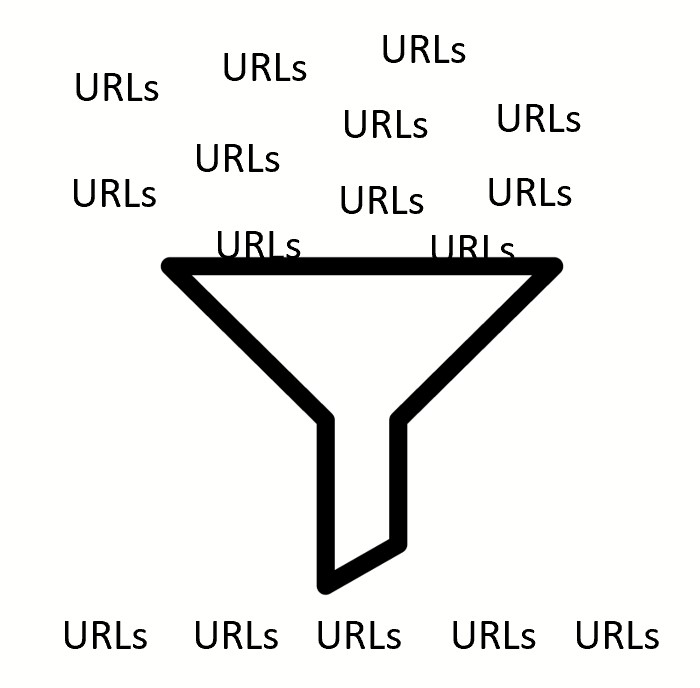
\includegraphics[totalheight=4.5cm]{filter.jpg}}
    \caption{URL Filter}
    \label{fig:verticalcell}
\end{figure}
%-----

Before that I loaded an environment variable and used the method re.compile() to compile the regex.
% Image
\begin{figure}[tph!]
\centerline{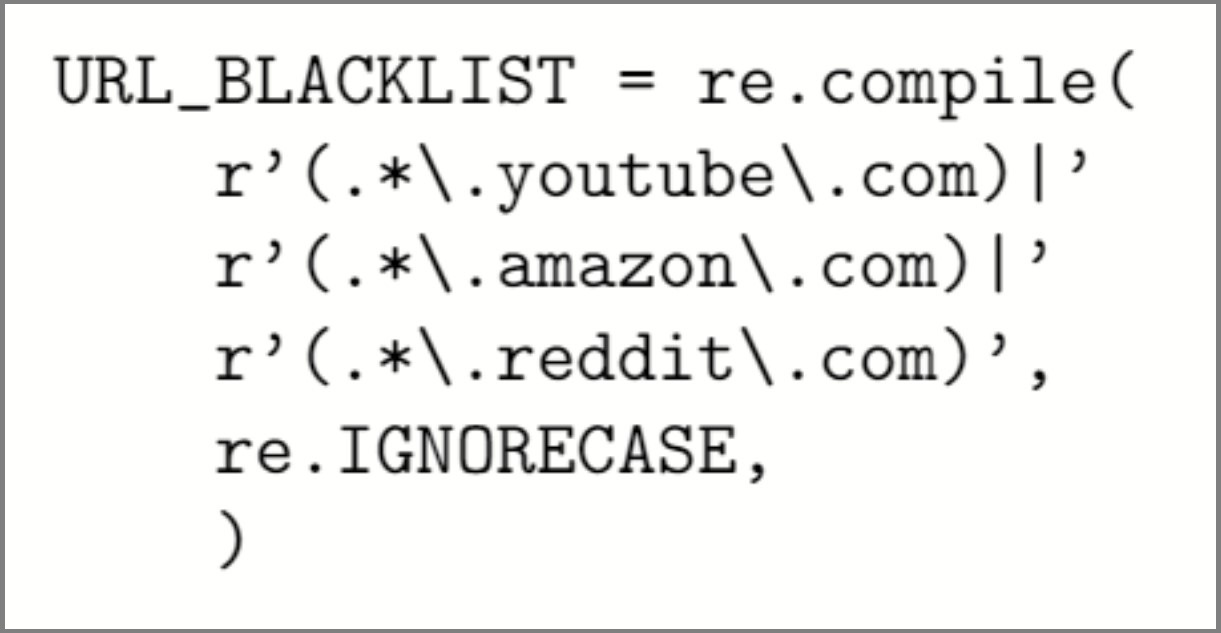
\includegraphics[totalheight=3cm]{code1.jpg}}
    \caption{Regex compilation}
    \label{fig:verticalcell}
\end{figure}
%-----

After that I created a method to exclude any URL that was in blacklist using generator comprehensions. 

% Image
\begin{figure}[tph!]
\centerline{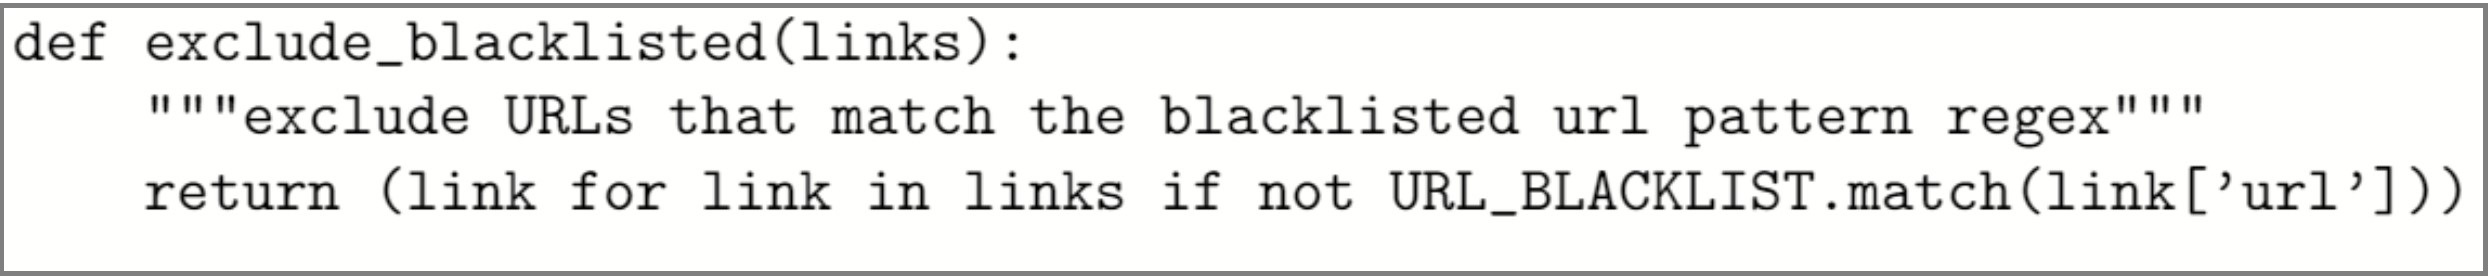
\includegraphics[totalheight=1cm]{code2.jpg}}
    \caption{Method using generator comprehension}
    \label{fig:verticalcell}
\end{figure}
%-----

Finally, I had one more challenge. I needed to find the perfect place to call this method, as links can only get loaded in a couple of places. Adding links from a new import source, parsing an existing output/links.json index file, or reading an individual json file. So I found a method which is executed before these three methods are called. 

\subsection{Code quality}

First of all, in the begging of my contribution process I tried to read as much code as I could in order to understand the best practises. I underlined naming principles that where adopted on the project, but also the number of empty lines they use between their methods etc. By doing this I managed to contribute code that suits the project.

Further more, I wrote descriptive comments to my methods and variables. 
% Image
\begin{figure}[tph!]
\centerline{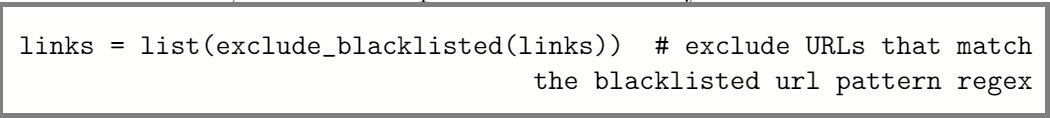
\includegraphics[totalheight=1cm]{code3.jpg}}
    \caption{Regex compilation}
    \label{fig:verticalcell}
\end{figure}
%-----

Every method I wrote was well documented, so as to create reproducible and scaling code.

\subsection{Continuous Integration \& Testing}
The project has only Docker Cloud (ci/dockercloud)[2], which allowed me to manage the project in a container without exposing it to the rest of my system. Eventually all my commits passed this check. As far as testing is concerned, code responded positively, so my code was merged to the project!

% Image
\begin{figure}[tph!]
\centerline{
\includegraphics[totalheight=1cm]{merge.jpg}}
    \caption{Merge}
    \label{fig:verticalcell}
\end{figure}
%-----

\section{Project organization}
I worked with GitHub in my forked repository. I tried to make small commits at a time in order to be specific in their description. Also GitHub helped me retrieve previous versions when that was needed. Finally when I finished my work I created a pull request describing my changes and also mentioning the corresponding issue I was hoping to close. Bellow you can see my activity in GitHub:
% Image
\begin{figure}[tph!]
\centerline{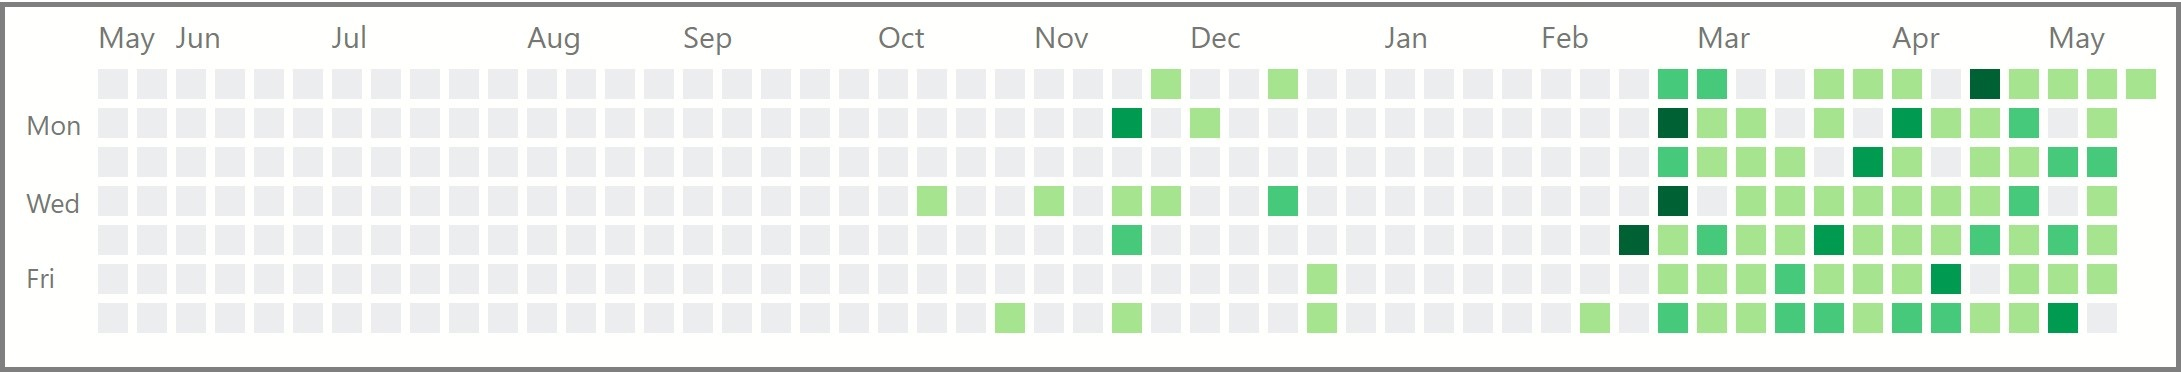
\includegraphics[totalheight=2cm]{github.jpg}}
    \caption{GitHub Activity}
    \label{fig:verticalcell}
\end{figure}
%-----
\newline
\section{Cooperation with the team}

From the beginning, I had excellent cooperation with the project owner Nick Sweeting. He surely helped me and introduced me to web archiving community. Also, I was constantly asking for feedback and code review and he was always willing to do so. Further than that, we also had a video call to talk about the project and my next task. I am very satisfied with our cooperation as I learned lots of things according to project organization and python programming. 

% Image
\begin{figure}[tph!]
\centerline{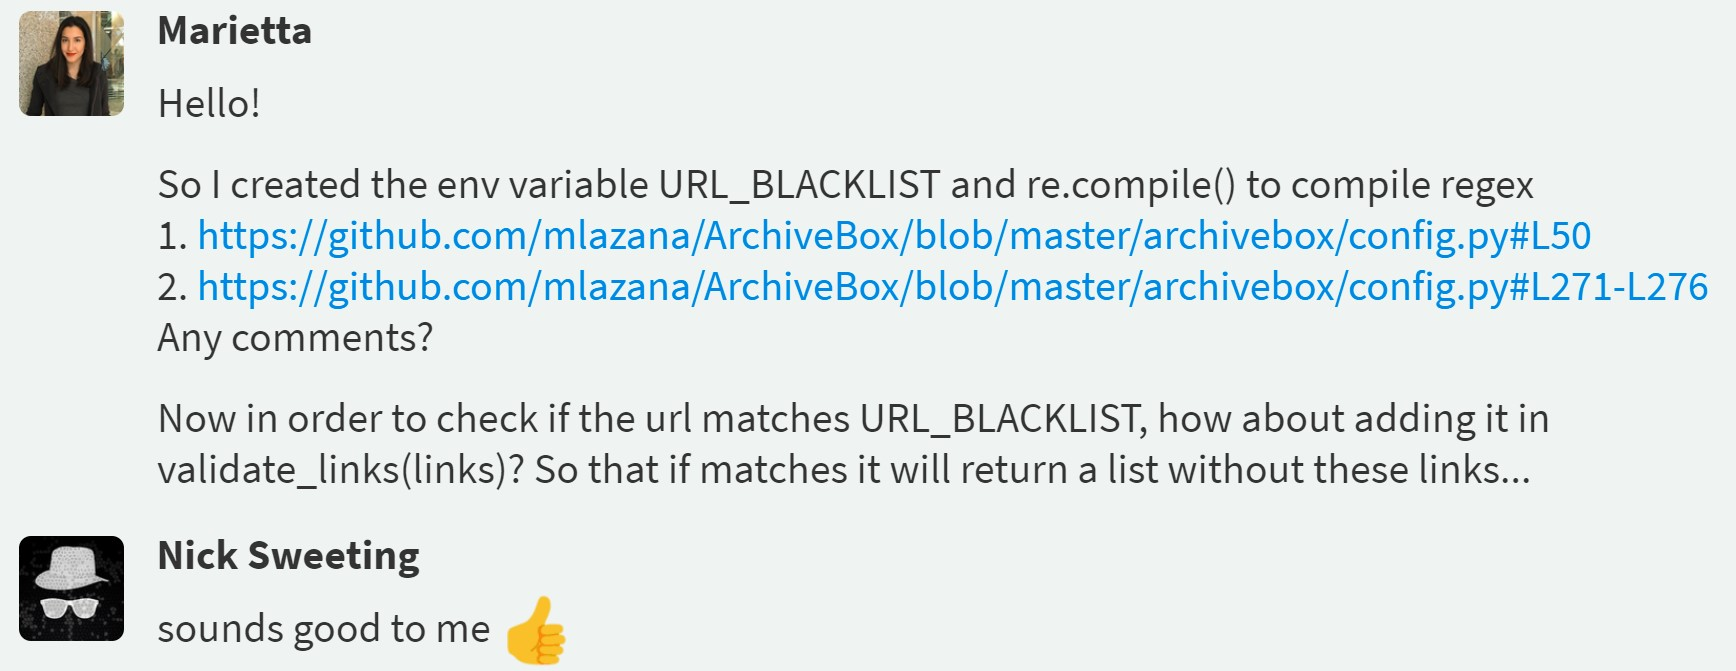
\includegraphics[totalheight=4.5cm]{cooperation.jpg}}
    \caption{Cooperation with project owner}
    \label{fig:verticalcell}
\end{figure}
%-----

\section{Conclusion}
My first contribution was an incredible journey as I broke out of my comfort zone and faced the real world of software engineering. Being involved in an open source project you always face your strengths and weaknesses, as you are not dealing only with yourself but also with an experienced development team.  Through my contribution process, I realised that being analytical and thorough will help me be deal with programming challenges. For me, a good software engineer has to combine code quality and team work which are the two key elements of open source community. That's the reason why I am not going to stop being a part of it. Lastly, I gained useful knowledge and I am ready to work hard to improve my skills in programming!

\section*{References}
[1] https://github.com/pirate/ArchiveBox 
\newline
[2]https://github.com/pirate/ArchiveBox/wiki/Docker

\end{document}
